\newif\ifimagen\imagentrue
\documentclass[10pt]{book}
\usepackage[width=5.5in,height=8.5in,hmarginratio=3:2,vmarginratio=1:1]{geometry}\usepackage[T1]{fontenc}\usepackage{textcomp}\usepackage{mathpazo}\usepackage{url}\usepackage{graphicx}\usepackage{amsmath}\usepackage{amsthm}\usepackage{amssymb}\usepackage{exercise}\usepackage{makeidx}\usepackage{setspace}\usepackage{hevea}\usepackage{upquote}\usepackage{appendix}\usepackage[italian]{babel}\usepackage[utf8x]{inputenc}\usepackage{latexsym}\usepackage[bookmarks]{hyperref}\newcommand{\thetitle}{Pensare in Python: Come pensare da Informatico}
\newcommand{\theversion}{Seconda Edizione, Versione 2.2.23}
\newcommand{\thedate}{}

\pagestyle{empty}
\thispagestyle{empty}
\begin{document}
\newtheorem{exercise}{Esercizio}[chapter]
\setcounter{chapter}{-1}
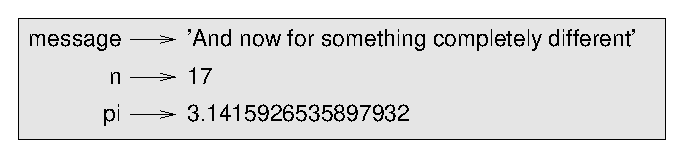
\includegraphics[scale=0.8]{./figs/state2.eps}
\clearpage% page: 0
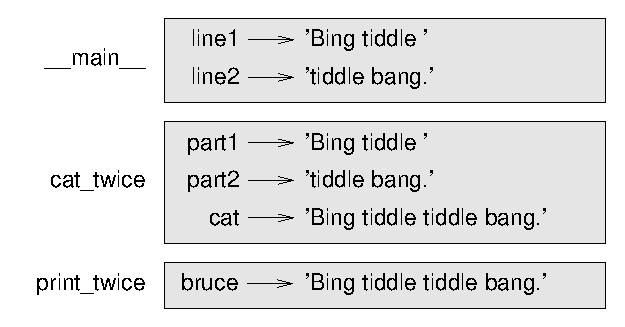
\includegraphics[scale=0.8]{./figs/stack.eps}
\clearpage% page: 1
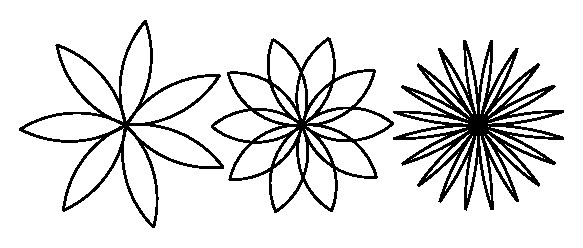
\includegraphics[scale=0.8]{./figs/flowers.eps}
\clearpage% page: 2
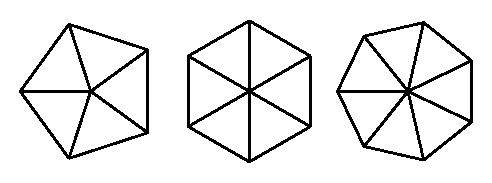
\includegraphics[scale=0.8]{./figs/pies.eps}
\clearpage% page: 3
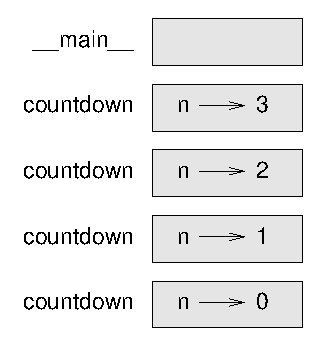
\includegraphics[scale=0.8]{./figs/stack2.eps}
\clearpage% page: 4
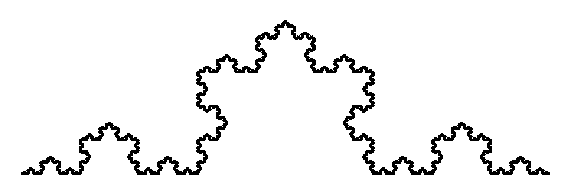
\includegraphics[scale=0.8]{./figs/koch.eps}
\clearpage% page: 5
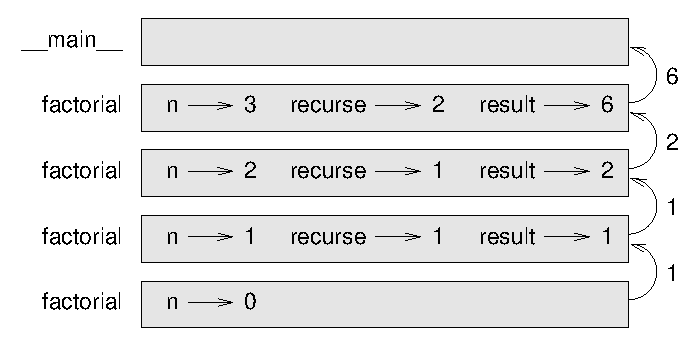
\includegraphics[scale=0.8]{./figs/stack3.eps}
\clearpage% page: 6

\includegraphics[scale=0.8]{./figs/assign2.eps}
\clearpage% page: 7
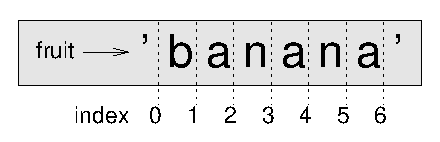
\includegraphics[scale=0.8]{./figs/banana.eps}
\clearpage% page: 8
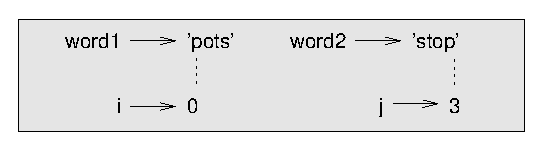
\includegraphics[scale=0.8]{./figs/state4.eps}
\clearpage% page: 9
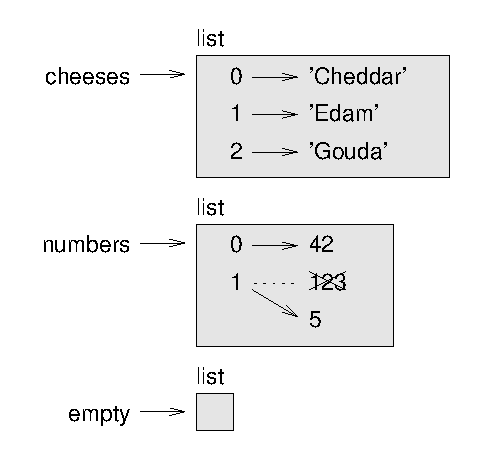
\includegraphics[scale=0.8]{./figs/liststate.eps}
\clearpage% page: 10
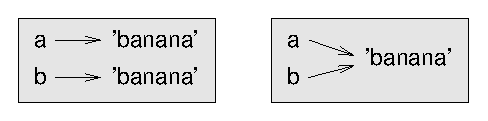
\includegraphics[scale=0.8]{./figs/list1.eps}
\clearpage% page: 11
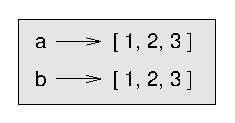
\includegraphics[scale=0.8]{./figs/list2.eps}
\clearpage% page: 12

\includegraphics[scale=0.8]{./figs/list3.eps}
\clearpage% page: 13
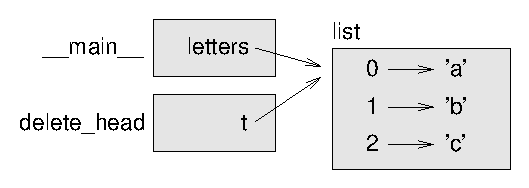
\includegraphics[scale=0.8]{./figs/stack5.eps}
\clearpage% page: 14
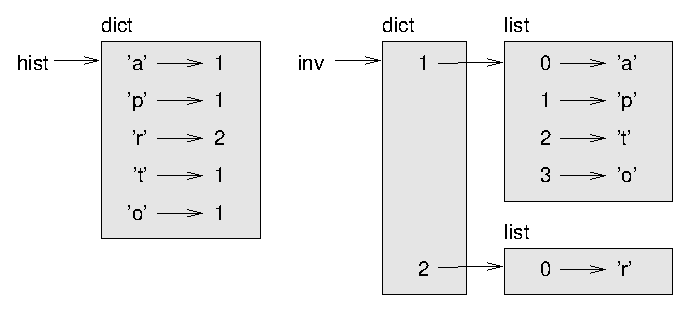
\includegraphics[scale=0.8]{./figs/dict1.eps}
\clearpage% page: 15
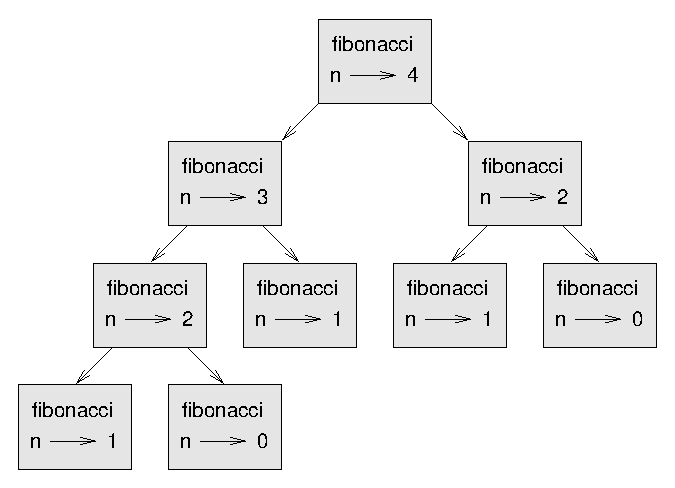
\includegraphics[scale=0.7]{./figs/fibonacci.eps}
\clearpage% page: 16
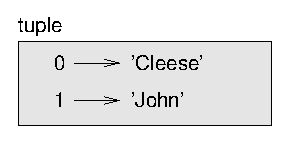
\includegraphics[scale=0.8]{./figs/tuple1.eps}
\clearpage% page: 17
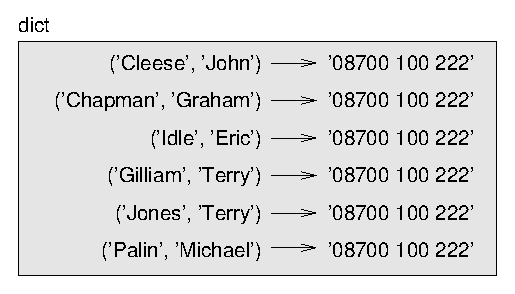
\includegraphics[scale=0.8]{./figs/dict2.eps}
\clearpage% page: 18
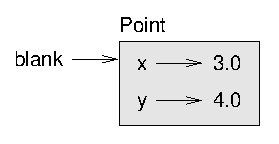
\includegraphics[scale=0.8]{./figs/point.eps}
\clearpage% page: 19
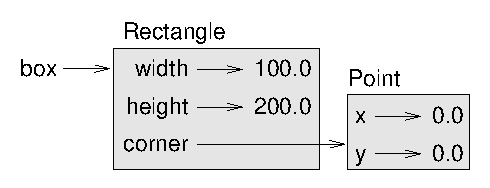
\includegraphics[scale=0.8]{./figs/rectangle.eps}
\clearpage% page: 20
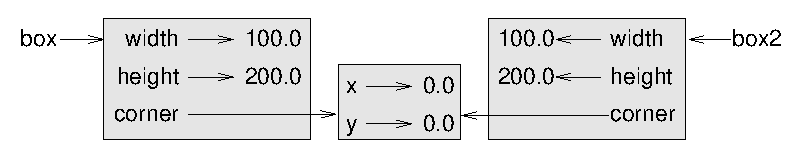
\includegraphics[scale=0.8]{./figs/rectangle2.eps}
\clearpage% page: 21
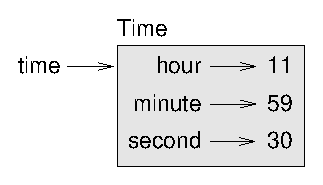
\includegraphics[scale=0.8]{./figs/time.eps}
\clearpage% page: 22
\newcommand{\mymapsto}{$\mapsto$}
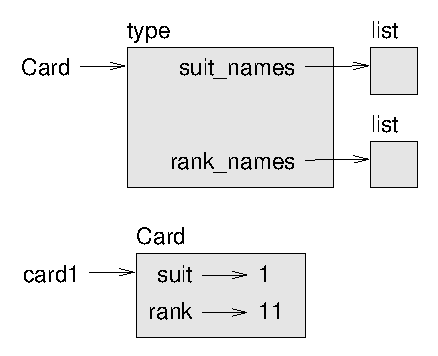
\includegraphics[scale=0.8]{./figs/card1.eps}
\clearpage% page: 23
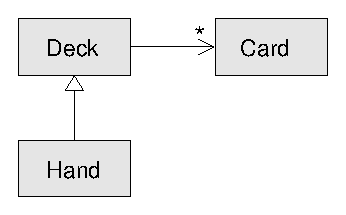
\includegraphics[scale=0.8]{./figs/class1.eps}
\clearpage% page: 24
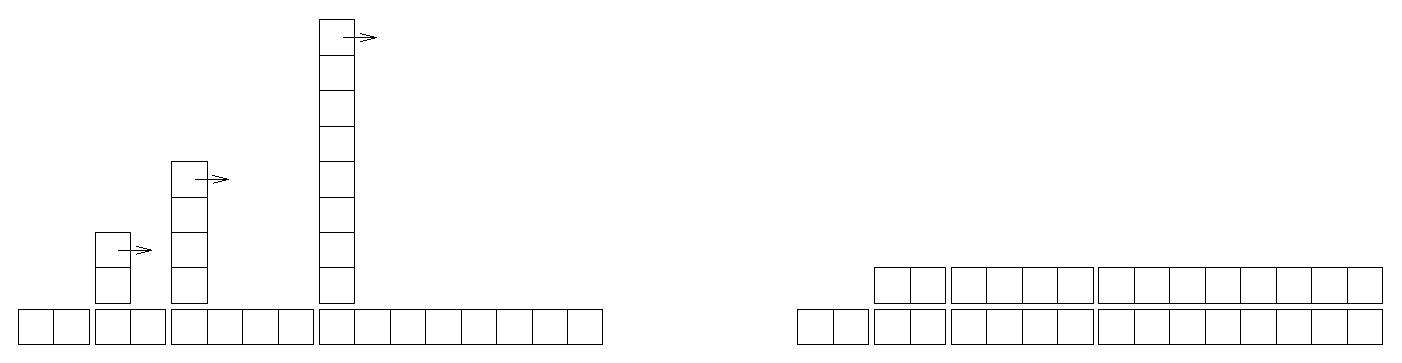
\includegraphics[scale=0.6]{./figs/towers.eps}
\clearpage% page: 25
%Options: 
\end{document}
